\documentclass[border=12pt]{standalone}
\usepackage{amsmath}
\usepackage{tikz}
\usetikzlibrary{arrows.meta}
\usepackage{xcolor}
\definecolor{weeknavy}{HTML}{243B53}
\definecolor{weekblue}{HTML}{6E8FB3}
\definecolor{weeksage}{HTML}{7AA69B}
\begin{document}
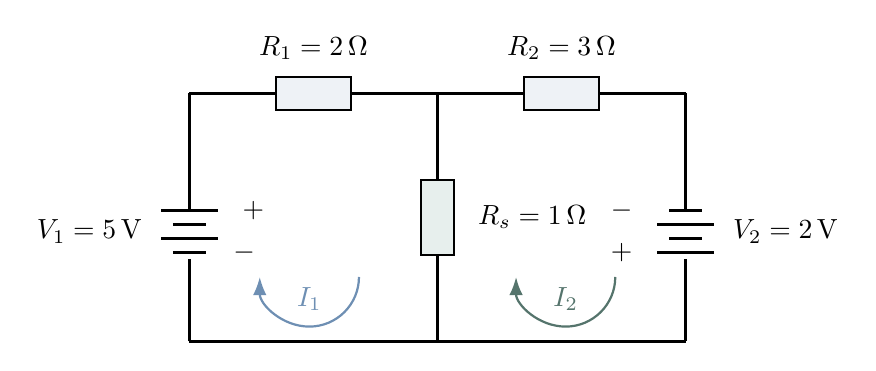
\begin{tikzpicture}[>=Latex,thick,scale=1.05]
% Two-loop DC resistor circuit. Long battery plate is positive.
\draw (0,0)--(3,0) (0,0)--(0,1.00);
\draw[line width=1.1pt] (-0.20,1.08)--(0.20,1.08);
\draw[line width=1.1pt] (-0.34,1.24)--(0.34,1.24);
\draw[line width=1.1pt] (-0.20,1.42)--(0.20,1.42);
\draw[line width=1.1pt] (-0.34,1.58)--(0.34,1.58);
\draw (0,1.58)--(0,3) (0,3)--(1.05,3);
\draw[fill=weekblue!12] (1.05,2.80) rectangle (1.95,3.20);
\draw (1.95,3)--(3,3);
\draw (3,0)--(6,0) (6,0)--(6,1.00);
\draw[line width=1.1pt] (5.66,1.08)--(6.34,1.08);
\draw[line width=1.1pt] (5.80,1.24)--(6.20,1.24);
\draw[line width=1.1pt] (5.66,1.42)--(6.34,1.42);
\draw[line width=1.1pt] (5.80,1.58)--(6.20,1.58);
\draw (6,1.58)--(6,3) (3,3)--(4.05,3);
\draw[fill=weekblue!12] (4.05,2.80) rectangle (4.95,3.20);
\draw (4.95,3)--(6,3);
\draw (3,0)--(3,1.05);
\draw[fill=weeksage!18] (2.80,1.05) rectangle (3.20,1.95);
\draw (3,1.95)--(3,3);
\draw (1.5,3.28) node[above] {$R_1=2\,\Omega$};
\draw (4.5,3.28) node[above] {$R_2=3\,\Omega$};
\draw (3.20,1.5) node[right=5pt] {$R_s=1\,\Omega$};
\draw (-0.45,1.33) node[left] {$V_1=5\,\mathrm{V}$};
\draw (0.45,1.58) node[right=2pt] {$+$};
\draw (0.34,1.08) node[right=2pt] {$-$};
\draw (6.45,1.33) node[right] {$V_2=2\,\mathrm{V}$};
\draw (5.55,1.08) node[left=2pt] {$+$};
\draw (5.55,1.58) node[left=2pt] {$-$};
\draw[->,weekblue] (2.05,0.78) arc[start angle=0,end angle=-180,radius=0.60] node[midway,above=2pt] {$I_1$};
\draw[->,weeksage!70!black] (5.15,0.78) arc[start angle=0,end angle=-180,radius=0.60] node[midway,above=2pt] {$I_2$};
\end{tikzpicture}
\end{document}
